\documentclass[
  ukrainian,
  simple,
  floatsection,
]{eskdnaukvd}

%%% Length calculations
\usepackage{calc}
%%%

%%% Math Typesetting
\usepackage{unicode-math}
\setmathfont{STIX Two Math}
\usepackage{IEEEtrantools}
%%%

%%% Language configuration
\usepackage{polyglossia}
\setdefaultlanguage{ukrainian}
\setotherlanguage{english}
%%%

%%% Font configuration
\setmainfont{STIX Two Text}
\setsansfont{IBM Plex Sans}
\setmonofont{IBM Plex Mono}
%%%

%%% List settings
\usepackage{enumitem}
\setlist[enumerate]{
  label*      = {\arabic*.},
  left        = \parindent,
  topsep      = 0\baselineskip,
  parsep      = 0\baselineskip,
  noitemsep, % override itemsep
}
% List settings for levels 2–4
\setlist[enumerate, 2, 3, 4]{
  label*      = {\arabic*.},
  left        = 0em,
  topsep      = 0\baselineskip,
  parsep      = 0\baselineskip,
  noitemsep, % override itemsep
}

\setlist[itemize]{
  label*      = {—},
  left        = \parindent,
  topsep      = 0\baselineskip,
  parsep      = 0\baselineskip,
  itemsep     = 1\baselineskip,
  noitemsep, % override itemsep
}

\setlist[description]{
  font        = {\rmfamily\upshape\bfseries},
  topsep      = 1\baselineskip,
  parsep      = 0\baselineskip,
  itemsep     = 0\baselineskip,
}

\newlist{litlist}{enumerate}{1}
\setlist[litlist]{
  label* = {\arabic*.},
  left = 0em,
}
%%%

%%% Code formatting settings
\newmintinline[minttext]{text}{%
}
%%%

%%% SI units typesetting
\usepackage{siunitx}
\sisetup{
  output-decimal-marker = {,},
  exponent-product      = {\cdot},
  inter-unit-product    = \ensuremath{{} \cdot {}},
  per-mode              = symbol,
}
%%%

%%% Drawing
\usepackage{tikz}
\usetikzlibrary{automata} % System state diagram
\usetikzlibrary{positioning}
\usetikzlibrary{shapes}
\usetikzlibrary{arrows.meta} % Stealth arrow tips
\usetikzlibrary{shapes.multipart} % Multipart rectangles for queue diagrams

%%%

%%% Define width grid
\newlength{\gridunitwidth}
\setlength{\gridunitwidth}{\textwidth / 12}
%%%

%%% GOST strings
\ESKDdepartment{Національний авіаційний університет}
\ESKDclassCode{}
% \ESKDtitle{Офісна локальна комп'ютерна мережа}
%\ESKDdocName{Курсова робота}
\ESKDsignature{НАУ~20 0224000 ПЗ}
\ESKDauthor{Клокун~В.\,Д.}
% \ESKDtitleApprovedBy{Керівник роботи}{Масловський Б.\,Г.}
\ESKDchecker{Масловський Б.\,Г.}
\ESKDcolumnIX{ФККПІ СП-425}
% \ESKDapprovedBy{Жуков І.\,А.}
%%%

%%% Define ESKD styles
\ESKDdefaultStyle{nauplain}
%%%

%%% Links and hyperreferences

% Support and define colors
\usepackage{xcolor}
\definecolor{lightblue}{HTML}{03A9F4}
\definecolor{red}{HTML}{F44336}
%

\usepackage{hyperref}
\hypersetup{
  bookmarksnumbered = true,
  colorlinks      = false,
  linkbordercolor = red,
  urlbordercolor  = lightblue,
  pdfborderstyle  = {/S/U/W 1.5},
}
%%%

\begin{document}

  \begin{titlepage}
    \ESKDthisStyle{title}
    \begin{center}
      Міністерство освіти і~науки України\\
      Національний авіаційний університет\\
      Факультет кібербезпеки, комп'ютерної та~програмної інженерії\\
      Кафедра комп'ютеризованих систем управління

      \vspace{\fill}
      Курсовий проект\\
      з~дисципліни~«Технології проектування комп'ютерних систем»\\
      Варіант №~2


      \vspace{\fill}


      \begin{flushleft}
      Виконавець: \hfill СП-425, Клокун В.\,Д.\\
      \end{flushleft}

      \vspace{\fill}

      Київ 2020
    \end{center}
  \end{titlepage}

  \newpage
  % Fix ESKDX page counter to include the title page
  \setcounter{page}{2}

  \ESKDthisStyle{nausection}
  \tableofcontents

  \section*{Постановка задачі}
  \addcontentsline{toc}{section}{Постановка задачі}
  \ESKDthisStyle{nausection}
    Необхідно побудувати математичну модель системи масового обслуговування для~комп’ютерної системи та~визначити показники ефективності її~функціонування.

    До~комп’ютерної системи надходить найпростіший потік завдань з~параметром~$\lambda$. Час~обслуговування одного завдання процесором розподілений за~експоненціальним законом з~параметром~$\mu$. Комп’ютерна система може мати один або~декілька процесорів~$m$, а~також може мати накопичувач (буфер) для~завдань~$K$.

    Побудувати аналітичну модель та~визначити показники ефективності функціонування: стаціонарні ймовірності перебування в~системі~$k$~завдань, ймовірність того, що~завдання потрапить в~чергу і~т.д.

    Для~аналізу системи використати \textenglish{QTS plus EXEL}, отримати показники функціонування системи та~порівняти їх~з~аналітичними. Проаналізувати отримані результати.

    Параметри системи, яку~необхідно дослідити, надані у~завданні за~варіантом~(табл.~\ref{tab:task}).

    \begin{table}[!htbp]
      \newlength{\tmptabcolwidth}
      \setlength{\tmptabcolwidth}{9 \gridunitwidth / 4}
      \caption{Параметри системи, яку~необхідно змоделювати за~варіантом}
      \label{tab:task}
      \begin{tabular}{
        |v{3 \gridunitwidth - 2\tabcolsep}
        *{4}{|n{\tmptabcolwidth - 2\tabcolsep}}
        |
      }
        \hline
          № варіанта & $\lambda$ & $\mu$ & $m$ & $K$ \\
        \hline
          2 & \num{0.1} & \num{0.2} & 3 & $\infty$ \\
        \hline
      \end{tabular}
    \end{table}

  \section{Побудова математичної моделі}
  \ESKDthisStyle{nausection}

    \subsection{Структурна схема системи}
      Щоб~наочно представити модельовану систему, необхідно побудувати її~структурну схему~(рис.~\ref{fig:struct-diagram}).

      \begin{figure}[!htbp]
        \centering
        \begin{tikzpicture}[
            font = {\small},
            phantom/.style = {
            },
            queue/.style = {
              draw,
              rectangle split,
              rectangle split horizontal,
              rectangle split parts = 3,
              minimum height = 1\gridunitwidth,
              minimum width = 1\gridunitwidth,
            },
            processor/.style = {
              draw,
              rectangle,
              minimum height = 1\gridunitwidth,
              minimum width = 1\gridunitwidth,
            },
            >=Stealth,
        ]
          \node [] (src) {};

          \node [
            queue,
            right = 3 \gridunitwidth of src,
            label = Черга,
          ] (q) {};

          \node [
            processor,
            anchor = north west,
            right = \gridunitwidth of q.east,
          ] (m2) {$m_2$};

          \node [
            processor,
            above = 0.5 \gridunitwidth of m2.north,
            label = {Процесори},
          ] (m1) {$m_1$};

          \node [
            processor,
            below = 0.5 \gridunitwidth of m2.south,
          ] (m3) {$m_3$};

          \node [
            coordinate,
            right = 1\gridunitwidth of m2.east,
          ] (dst-converge) {};

          \node [
            right = 3\gridunitwidth of dst-converge.east,
          ] (dst) {};

          % Arrows
          \path [->] (src) edge node [above] {Вхідний потік} (q)
                     (q.east) edge (m1.west)
                              edge (m2.west)
                              edge (m3.west);
          \path [draw] (m1.east) -| (dst-converge);
          \path [draw] (m2.east) -- (dst-converge);
          \path [draw] (m3.east) -| (dst-converge);
          \path [draw]
            (dst-converge)
            edge [->] node [above] {Вихідний потік}
            (dst);

        \end{tikzpicture}
        \caption{Структурна схема модельованої схеми}
        \label{fig:struct-diagram}
      \end{figure}

    \subsection{Граф переходів станів системи}
      Стани модельованої системи масового обслуговування можна представити у~вигляді графа переходів станів системи~(рис.~\ref{fig:state-diag}).

      \begin{figure}[!htbp]
        \centering
        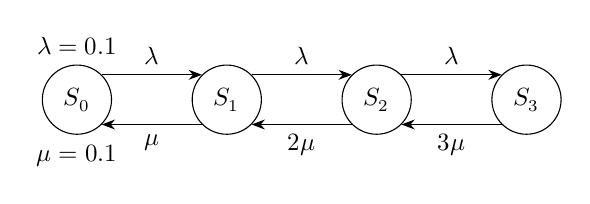
\begin{tikzpicture}[
            font = {\small},
            >=Stealth,
        ]
          \node [
            state,
            label={$\lambda = \num{0.1}$},
            label={below:$\mu = \num{0.1}$},
          ] (s0) {$S_0$};
          \node [state] (s1) [right = 1 \gridunitwidth of s0] {$S_1$};
          \node [state] (s2) [right = 1 \gridunitwidth of s1] {$S_2$};
          \node [state] (s3) [right = 1 \gridunitwidth of s2] {$S_3$};

          % Edges
          \path [->] (s0.north east) edge node [above] {$\lambda$} (s1.north west)
                     (s1.south west) edge node [below] {$\mu$} (s0.south east)
                     (s1.north east) edge node [above] {$\lambda$} (s2.north west)
                     (s2.south west) edge node [below] {$2 \mu$} (s1.south east)
                     (s2.north east) edge node [above] {$\lambda$} (s3.north west)
                     (s3.south west) edge node [below] {$3 \mu$} (s2.south east);
        \end{tikzpicture}
        \caption{Граф переходів станів системи}
        \label{fig:state-diag}
      \end{figure}

      Представлений граф переходів показує, що~система може знаходитись у~таких станах:
      \begin{enumerate}
        \item Стан~$S_0$~— усі~канали системи вільні.
        \item Стан~$S_1$~— система використовує 1 канал.
        \item Стан~$S_2$~— система використовує 2 канали.
        \item Стан~$S_3$~— система використовує 3 канали.
      \end{enumerate}
      На~початку система знаходиться у~стані~$S_0$. Коли в~систему надходить потік заявок з~інтенсивністю~$\lambda$, він~переводить її~зі~стану~$S_0$ в~стан~$S_1$. Коли система зможе обробити заявки, тобто надасть потік обслуговування~$\mu$, він~поверне систему зі~стану~$S_1$ до~стану~$S_0$. Збільшення інтенсивності потоку на~$\lambda$ на~кожному стані~$S_i$ буде переводити його у~стан~$S_{i+1}$, де~$i \in {0, 1, 2}$. Аналогічно, якщо у~стані буде збільшуватись інтенсивність потоку~$\mu$, наприклад~$i \cdot \mu$, він~переведе систему зі~стану~$S_i$ до~стану~$S_{i-1}$, де~$i \in \{1, 2, 3\}$.

      \subsection{Математичні моделі для~побудови моделі}
        Щоб~побудувати необхідну модель системи масового обслуговування, необхідно визначити її~математичну модель. Математична модель заданої системи масового обслуговування має~такі параметри:\\
        \begin{tabular}{
          n{1\gridunitwidth - 2\tabcolsep}
          @{ — }
          v{11\gridunitwidth - 2\tabcolsep}
        }
          $\lambda$ & інтенсивність вхідного потоку задач, тобто кількість заявок, які~надходять у~систему за~одиницю часу.\\
          $\mu$ & інтенсивність, з~якою процесор обслуговує задачі, тобто час~обслуговування однієї задачі.\\
          $m$ &  кількість процесорів у~системі, які~можуть обслуговувати задачі. Також називаються каналами.\\
          $K$ & розмір накопичувача (буфера) завдань, який показує кількість задач, які~можуть одночасно перебувати в~черзі.
        \end{tabular}

  \section{Аналітичне визначення показників ефективності функціонування}
  \ESKDthisStyle{nausection}
    Перед тим, як~приступити до~моделювання, варто визначити деякі її~показники аналітично, щоб~розуміти, наскільки адекватно відображає реальність комп'ютерне моделювання. \emph{Навантаженість системи}~$\rho$ показує, скільки відсотків ресурсів системи використовується і~обчислюється так:
    \begin{IEEEeqnarray*}{l}
      \rho = \frac{\lambda}{m \cdot \mu} \cdot 100\%
           = \frac{\num{0.1}}{3 \cdot \num{0.1}} \cdot 100\%
           = \num{33.3} \%
    \end{IEEEeqnarray*}

    \emph{Середній час~обслуговування} є~вхідним параметром для~моделі. Він~позначається як~$1 / \mu$ і~аналогічно обчислюється:
    \begin{IEEEeqnarray*}{l}
      \frac{1}{\mu} = \frac{1}{\num{0.1}} = 10.
    \end{IEEEeqnarray*}

    \emph{Доля часу простою системи} (або~ймовірність того, що~процесори вільні) показує, яку~частку часу процесори проводять, не~оброблюючи запити. Вона обчислюється так:
    \begin{IEEEeqnarray*}{l}
      \frac{1}{
        \displaystyle\sum_{i=0}^{m} \frac{p^m}{m!}
      }
      =
      \frac{1}{
        \displaystyle\frac{1^0}{0!}
        + \frac{1^1}{1!}
        + \frac{1^2}{2!}
        + \frac{1^3}{3!}
        + \frac{1^{3+1}}{3! (3-1)}
      } = \num{0.364},
    \end{IEEEeqnarray*}
    де~$p = \lambda / \mu = 1$~— інтенсивність навантаження.

  \section{Комп'ютерне моделювання системи}
  \ESKDthisStyle{nausection}

    \subsection{Короткий опис пакету~\textenglish{\allcaps{QTS} plus \allcaps{EXEL}}}
      Пакет~\textenglish{\allcaps{QTS} plus \allcaps{EXEL}}~— це~додаток для~офісного пакету~\textenglish{Microsoft Excel}, який розповсюджується окремо, але~безкоштовно. Він~дозволяє моделювати системи масового обслуговування 7~різних категорій. Пакет розповсюджується у~вигляді~\textenglish{\allcaps{ZIP}}-архіву, який містить файли макросів~\textenglish{Microsoft Excel}. Щоб~запустити програму, необхідно відкрити файл~\textenglish{QtsPlus.xls} і~послідовно виконувати вказівки.

    \subsection{Визначення показників функціонування системи за~допомогою пакету~\textenglish{\allcaps{QTS} plus \allcaps{EXEL}}}
      Щоб~визначити показники функціонування системи, необхідно запустити пакет~\textenglish{\allcaps{QTS} plus \allcaps{EXEL}}. Для~цього відкриваємо файл~\textenglish{QtsPlus.xls}. З'явиться вікно налаштування моделювання~(рис.~\ref{fig:qts-main}).

      \begin{figure}[!htbp]
        \centering
        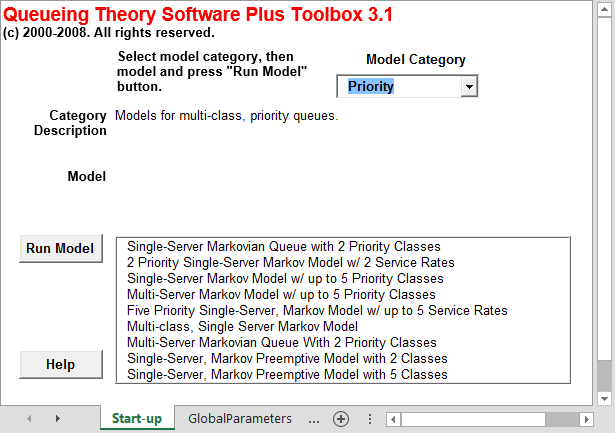
\includegraphics[height = 10 \baselineskip]{./assets/01-qts-main.png}
        \caption{Стартове вікно налаштування моделювання в~пакеті~\textenglish{\allcaps{QTS} plus \allcaps{EXEL}}}
        \label{fig:qts-main}
      \end{figure}

      Тепер необхідно обрати модель, яку~необхідно моделювати за~завданням варіанту. Для~цього у~вікні налаштування моделювання у~випадаючому меню~«\textenglish{Model Category}» необхідно обрати варіант~«\textenglish{Multi-Server}» і~модель~«\textenglish{M/M/C: Poisson Arrivals to Multiple Exponential Servers}»~(рис.~\ref{fig:qts-model-sel}).

      \begin{figure}[!htbp]
        \centering
        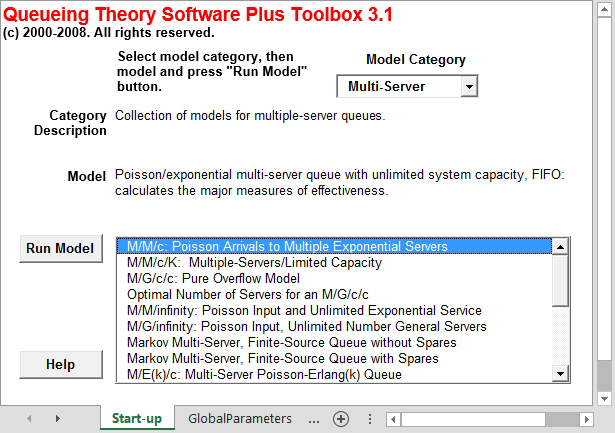
\includegraphics[height = 9 \baselineskip]{./assets/02-qts-model-sel.png}
        \caption{Вікно вибору моделі в~пакеті~\textenglish{\allcaps{QTS} plus \allcaps{EXEL}}}
        \label{fig:qts-model-sel}
      \end{figure}

      Коли модель обрана, необхідно запустити моделювання. Для~цього у~вікні вибору моделі необхідно натиснути кнопку~«\textenglish{Run Model}». Відкриється вікно налаштування обраної моделі~(рис.~\ref{fig:qts-model-main}). У~відкритому вікні вводимо параметри математичної моделі. Коли параметри введені, моделювання відбудеться автоматично і~результати моделювання оновляться~(табл.~\ref{tab:qts-model-res-num}).

      \begin{figure}[!htbp]
        \centering
        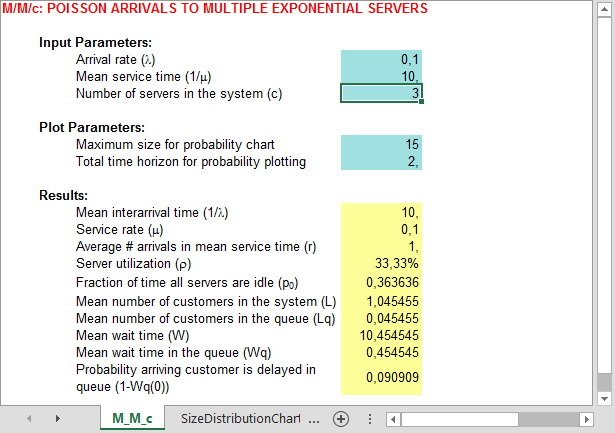
\includegraphics[height = 9 \baselineskip]{./assets/03-qts-model-res-num.png}
        \caption{Вікно налаштування обраної моделі в~пакеті~\textenglish{\allcaps{QTS} plus \allcaps{EXEL}}}
        \label{fig:qts-model-main}
      \end{figure}

      \begin{table}[!htbp]
        \centering
        \caption{Результати моделювання заданої системи масового обслуговування}
        \label{tab:qts-model-res-num}
        \begin{tabular}{
          |v{10\gridunitwidth - 2\tabcolsep}
          |n{2\gridunitwidth - 2\tabcolsep}
          |
        }
          \hline
          Параметр & Значення \\
          \hline
          Середній час~прибуття задачі~$1 / \lambda$ &  10 \\
          Середній час~обробки задачі~$\mu$ &  \num{0.1} \\
          Середня кількість нових задач за~середній час~обробки~$r$ & 1\\
          Завантаження процесорів~$\rho$ & \num{33.33}\% \\
          Частка часу повного простою процесорів~$p_0$ & \num{0.363636} \\
          Середня кількість заявок у~системі~$L$ & \num{1.045455} \\
          Середня кількість заявок у~черзі~$L_q$ & \num{0.045455} \\
          Середній час~очікування~$W$ & \num{10.454545} \\
          Середній час~очікування в~черзі~$W_q$ & \num{0.454545} \\
          Ймовірність, що~прибула заявка затримається в~черзі~$1 - W_q(0))$ & \num{0.090909}\\
          \hline
        \end{tabular}
      \end{table}

    \subsection{Візуалізація результатів, побудова залежностей ймовірнісно-часових характеристик від~певних параметрів}
      Пакет дозволяє візуалізувати результати моделювання, а~саме побачити графік густини ймовірностей, що~черга заявок матиме певний розмір, і~графік розподілу ймовірностей часу, проведеного в~черзі. Щоб~побачити графік густини ймовірностей, що~черга заявок матиме певний розмір~$n$, необхідно перейти у~сусідню вкладку~«\textenglish{SizeDistributionChart}»~(рис.~\ref{fig:qts-size-distr-chart}).

      \begin{figure}[!htbp]
        \centering
        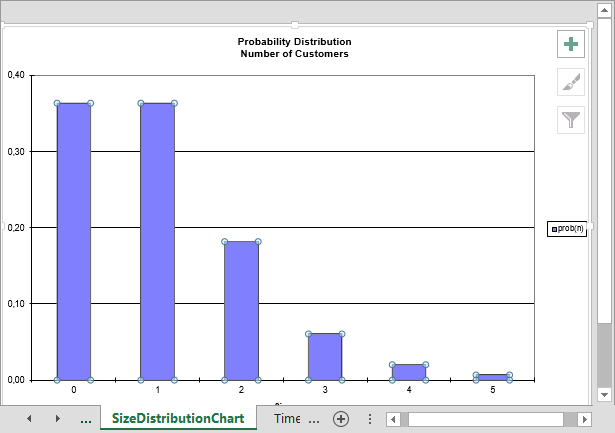
\includegraphics[height = 12 \baselineskip]{./assets/04-qts-model-res-graph-01.png}
        \caption{Графік густини ймовірностей, що~черга заявок матиме розмір~$n$ для~обраної моделі в~пакеті~\textenglish{\allcaps{QTS} plus \allcaps{EXEL}}}
        \label{fig:qts-size-distr-chart}
      \end{figure}

      Побудований графік показує, що~найбільш імовірно, що~система обслуговуватиме~$1—2$~заявки у~певний момент часу. Ймовірність обслуговування більшої кількості заявок зменшується за~експоненційним законом.

      Щоб~побачити графік розподілу ймовірностей часу, проведеного в~черзі, необхідно перейти у~вкладку~«\textenglish{TimeDistributionChart}»~(рис.~\ref{fig:qts-time-distr-chart}).

      \begin{figure}[!htbp]
        \centering
        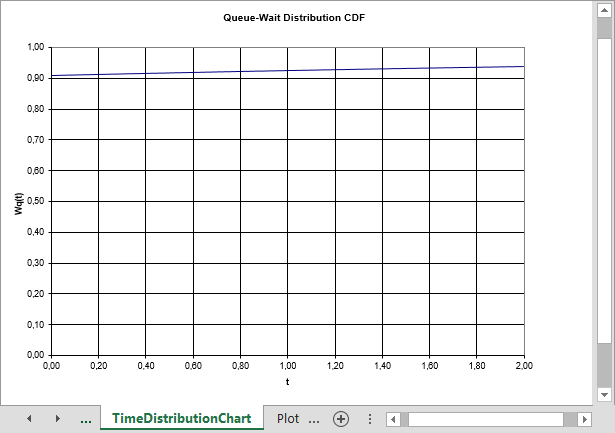
\includegraphics[height = 12 \baselineskip]{./assets/04-qts-model-res-graph-02.png}
        \caption{Графік розподілу ймовірностей часу~$t$, проведеного в~черзі, для~обраної моделі в~пакеті~\textenglish{\allcaps{QTS} plus \allcaps{EXEL}}}
        \label{fig:qts-time-distr-chart}
      \end{figure}

      Побудований графік показує, що~з~імовірністю~\num{0.9} нові заявки не~будуть затримуватись у~черзі, а~натомість будуть миттєво оброблені. Також видно, що~95\% заявок будуть оброблені не~довше, ніж~за~2~одиниці часу.

  \section{Аналіз та~інтерпретація результатів}
  \ESKDthisStyle{nausection}
    Виконуючи даний курсовий проект, була досліджена система масового обслуговування типу~$M/M/c/K$ з~параметрами~$m = 3$, $K = \infty$. Це~3-канальна однорідна експоненціальна система масового обслуговування без~буферизації (тому розмір буферу вважається нескінченним). У~ході виконання для~перевірки адекватності моделювання системи були обчислені аналітичні показники. Результати моделювання співпадають з~обчисленими аналітичними показниками, тому є~підстави вважати, що~моделювання достовірне.

    Результати моделювання показали, що~задана за~варіантом система масового обслуговування повністю справляється із~покладеним на~неї~навантаженням: найбільш імовірно, що~у~системі буде використовуватись менше каналів, ніж~у~ній~є, а~ймовірність використання усіх каналів менша за~\num{0.20}. Крім того, нові заявки дуже швидко оброблюються: переважна більшість заявок~(95\%) буде оброблена швидше, ніж~за~2~одиниці часу.

    Також під~час~аналітичного обчислення показників і~моделювання виявлено, що~система має~невеликі значення завантаженості~(\num{33.3}\%) і~великі частки часу простою~(\num{36}\%), що~підкреслює, що~задана система з~легкістю справляється із~покладеним навантаженням і~має~серйозний запас, а~тому її~ефективність і~утилізація знаходяться на~низькому рівні.

  \section*{Список використаної літератури}
  \addcontentsline{toc}{section}{Список використаної літератури}
  \ESKDthisStyle{nausection}

    \begin{litlist}
    \item \textit{Лаврусь О.\,Е., Міронов Ф.\,С}. Комп'ютерні мережі. Навчальний посібник. —~Кіровоград: \allcaps{ЦОП}~Авангард, 2008. —~146~с.
    \item \textit{Масловський Б.\,Г. Дрововозов В.\,І., Коба О.\,В}. Технології проектування ком\-п’\-ю\-тер\-них~систем. / Навчальний посібник. —~К.: \allcaps{НАУ}, 2015. —~500~с.
    \item \textit{Вишневский В.\,М}. Теоретические основы проектирования компьютерных сетей. —~М.: Техносфера, 2003. —~512~с.
    \end{litlist}

\end{document}
